\let\negmedspace\undefined
\let\negthickspace\undefined
\documentclass[journal]{IEEEtran}
\usepackage[a5paper, margin=10mm, onecolumn]{geometry}
\usepackage{lmodern} % Ensure lmodern is loaded for pdflatex
\usepackage{tfrupee} % Include tfrupee package

\setlength{\headheight}{1cm} % Set the height of the header box
\setlength{\headsep}{0mm}     % Set the distance between the header box and the top of the text

\usepackage{gvv-book}
\usepackage{gvv}
\usepackage{cite}
\usepackage{amsmath,amssymb,amsfonts,amsthm}
\usepackage{algorithmic}
\usepackage{graphicx}
\usepackage{textcomp}
\usepackage{xcolor}
\usepackage{txfonts}
\usepackage{listings}
\usepackage{enumitem}
\usepackage{mathtools}
\usepackage{gensymb}
\usepackage{comment}
\usepackage[breaklinks=true]{hyperref}
\usepackage{tkz-euclide} 
\usepackage{listings}                                      
\def\inputGnumericTable{}                                 
\usepackage[latin1]{inputenc}                                
\usepackage{color}                                            
\usepackage{array}                                            
\usepackage{longtable}
\usepackage{multicol}
\usepackage{calc}                                             
\usepackage{multirow}                                         
\usepackage{hhline}                                           
\usepackage{ifthen}                                           
\usepackage{lscape}
\begin{document}
	
	\bibliographystyle{IEEEtran}
	\vspace{3cm}
	
	\title{10.4.2.5}
	\author{EE24BTECH11064 - Harshil Rathan}
	% \maketitle
	% \newpage
	% \bigskip
	{\let\newpage\relax\maketitle}
	
	\renewcommand{\thefigure}{\theenumi}
	\renewcommand{\thetable}{\theenumi}
	\setlength{\intextsep}{10pt} % Space between text and floats
	
	
	\numberwithin{equation}{enumi}
	\numberwithin{figure}{enumi}
	\renewcommand{\thetable}{\theenumi}
	
	
\textbf{Question}:\\
The altitude of a right triangle is 7cm less than its base. If the hypotenuse is 13cm, find the other two sides 
\\
\textbf{Solution: }\\
We get the equation 
\begin{align}
    x^2 + (x-7)^2 = 13^2 
\end{align}
\begin{align}
     x^2-7x-60 =0
\end{align}
We can solve the above equation using fixed point iterations. First we separate $x$, from the above equation and make an update equation of the below sort.
\begin{align}
	x = g\brak{x} = \frac{x^2-60}{7}
\end{align}
Applying the above update equation on our equation, we get
\begin{align}
	x_{n+1}=\frac{x_n^2-60}{7}
\end{align}
Now we start with an initial guess $x_0 = 10 $\\
 But we realize that the updated values always approach infinity for any initial value. \\
Thus we will alternatively use Newton's Method for solving equations.
\begin{align}
	x_{n+1} = x_n - \frac{f\brak{x_n}}{f^{\prime}\brak{x_n}} 
\end{align}
Where we define $f\brak{x}$ as, 
\begin{align}
	f(x) = x^2 - 7x - 60 
\end{align}
\begin{align}
    f'(x) = 2x - 7
\end{align}
Thus, the new update equation is, 
\begin{align}
	x_{n+1} = x_n - \frac{x_n^2-7x_n-60}{2x_n-7 } 
\end{align}
Taking the initial guess as $x_0 = 10$, we can see that $x_n$ converges with x as,
\begin{align}
	x \approx 12.002
\end{align}
\begin{align}
    x = 12cm 
\end{align}
Alternatively, we can use the Secant method for solving equations.
\begin{align}
	x_{n+1} = x_n + f\brak{x_n}\frac{x_{n} -  x_{n-1}}{f(x_{n}) -  f(x_{n-1})}
\end{align}
The altitude is 
\begin{align}
    12 - 7 = 5cm 
\end{align}
The base is 12cm and the altitude is 5cm 
	\begin{figure}[h!]
		\centering
		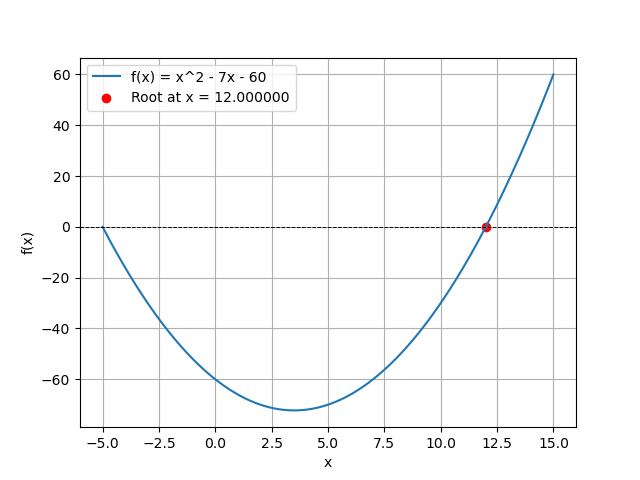
\includegraphics[width=\columnwidth]{figs/Figure_1.png}
	\end{figure}
	
\end{document}  
